\subsubsection{7-Segment Displays Parallel Port}

There are two parallel ports connected to the 7-segment displays on the \DEBoard~board, each of
which comprises a 32-bit write-only {\it Data} register. As indicated in 
Figure \ref{fig:segment_port}, the register at address {\sf 0xFF200020} 
drives digits {\it HEX3} to {\it HEX0}, and the register at 
address {\sf 0xFF200030} drives digits {\it HEX4} to
{\it HEX7}.  Data can be written into these two registers by using word operations. 
This data directly controls the segments of each display, according to
the bit locations given in Figure \ref{fig:segment_port}. The locations of segments 
6 to 0 in each seven-segment display on the DE2-115 board is illustrated on the right side of the
figure.

\begin{figure}[h!]
   \begin{center}
       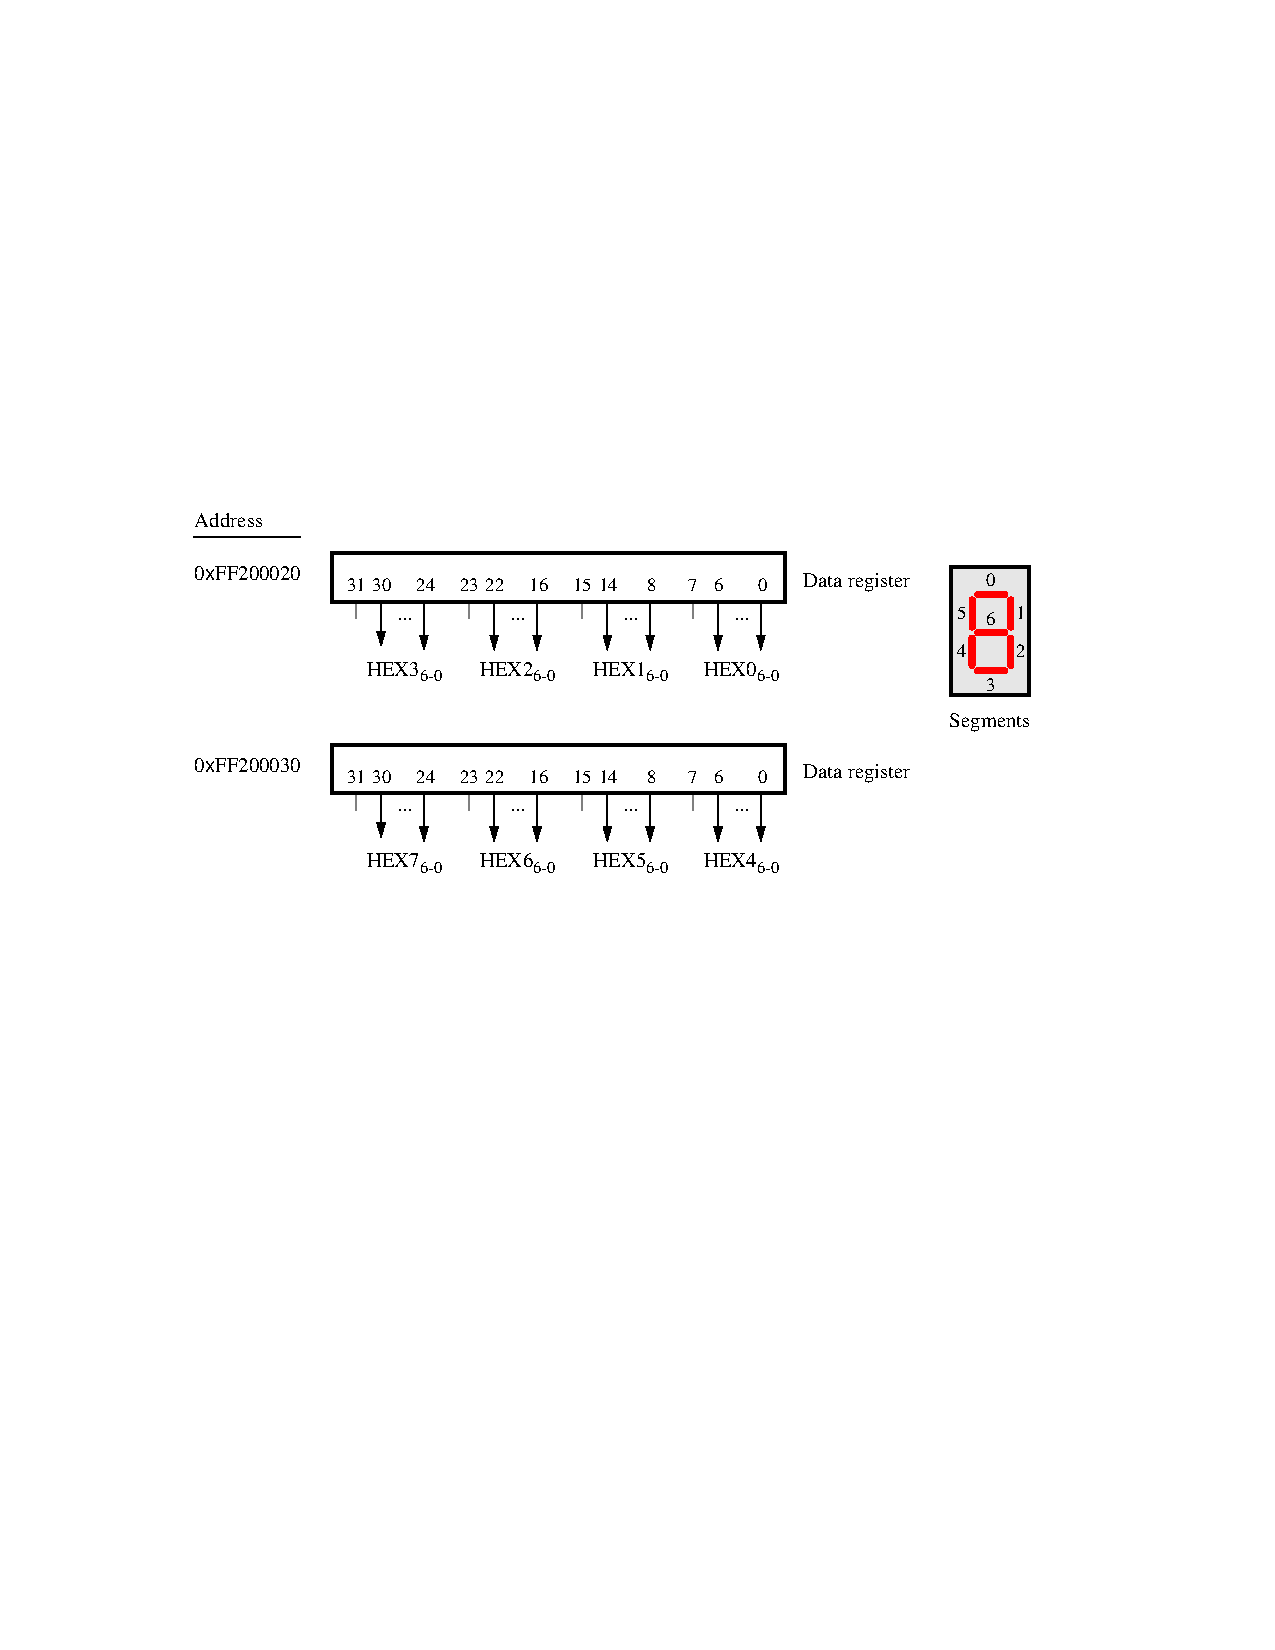
\includegraphics{../../../common/figs/FPGA_PP_7_Segs_8.pdf}
   \end{center}
   \caption{Bit locations for the 7-segment displays parallel ports.}
	\label{fig:segment_port}
\end{figure}